\PassOptionsToPackage{table}{xcolor}
\documentclass[10pt]{beamer}
\usepackage[english]{babel}

% Beamer theme
\usetheme{metropolis}

\usepackage{smartdiagram}
\usepackage{lstautogobble}
\usepackage{listings}
\usepackage{booktabs}
\usepackage[scale=2]{ccicons}%creative commons
\setbeamercovered{transparent}%invisible by default
\usepackage{array}
\newcolumntype{L}[1]{>{\raggedright\let\newline\\arraybackslash\hspace{0pt}}m{#1}}
\newcolumntype{C}[1]{>{\centering\let\newline\\arraybackslash\hspace{0pt}}m{#1}}
\newcolumntype{R}[1]{>{\raggedleft\let\newline\\arraybackslash\hspace{0pt}}m{#1}}

\usepackage{pgfplots}
\usepgfplotslibrary{dateplot}
\usepackage{tikz}
\usetikzlibrary{positioning,chains,fit,shapes,calc}
\usetikzlibrary{positioning,chains,fit,shapes,calc,automata,positioning}
\usepackage{fancyvrb}

% To include metapost files.
\usepackage{ifpdf}                        % To check if pdflatex is used.
\ifpdf
  \DeclareGraphicsRule{*}{mps}{*}{}
\fi

% Define path for images.
\graphicspath{{./}, {./Images/}}

% few useful commands
\providecommand{\ie}{i.\,e.}
\providecommand{\Ie}{I.\,e.}
\providecommand{\eg}{e.\,g.}
\providecommand{\Eg}{E.\,g.}

\providecommand{\mycomment}[1]{}

% Basic listing setting (eg, autogobble to remove left margin)
\lstset{basicstyle=\ttfamily, autogobble}

% metropolis template settings
\metroset{block=fill}
\metroset{titleformat frame=smallcaps}

\title{The comonadic smell of spreadsheets}
%\subtitle{}

\date{\today}
\author[Alessandro Candolini]{Alessandro Candolini}
%\institute{}
% \titlegraphic{\hfill\includegraphics[height=1.5cm]{logo/logo}}

\begin{document}

\maketitle

\begin{frame}[fragile]
  \begin{figure}
    \centering
    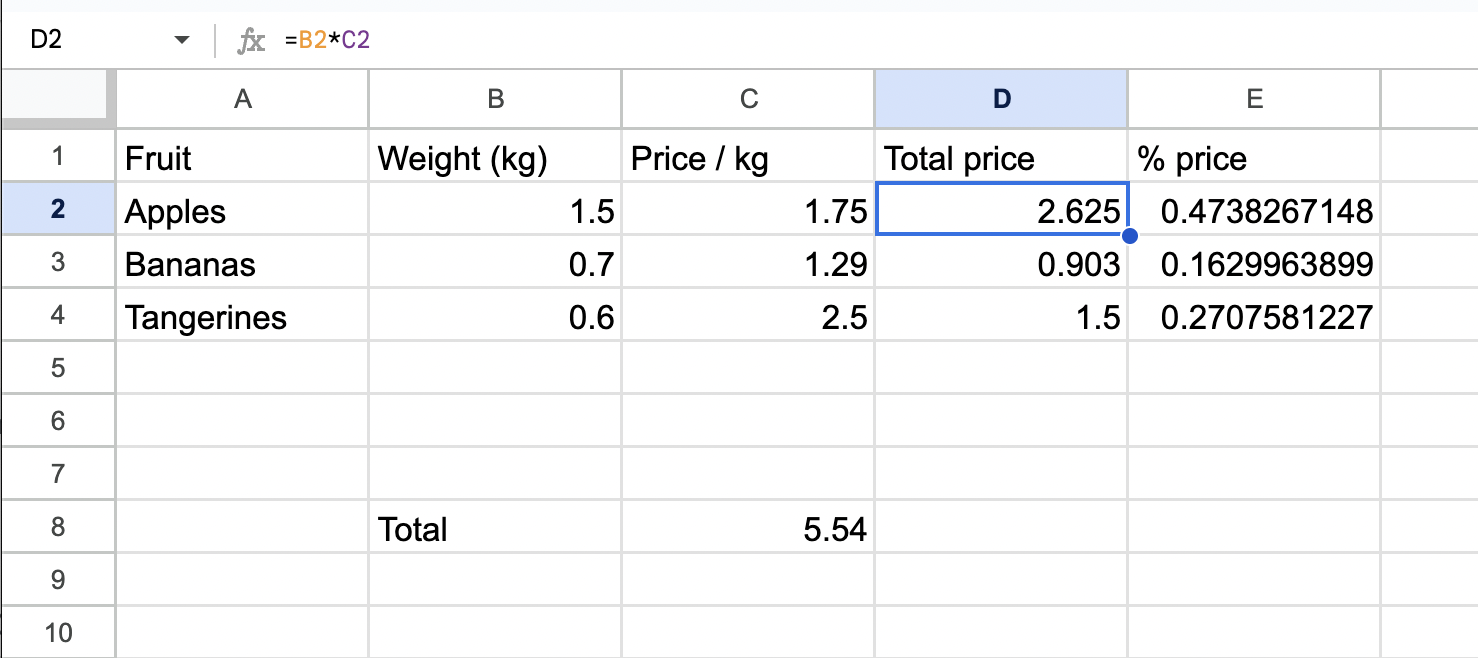
\includegraphics[width=.9\textwidth]{fruit1}
    \caption{Example of a 2D spreadsheet}
  \end{figure}
\end{frame}

\begin{frame}[fragile]
  \begin{figure}
    \centering
    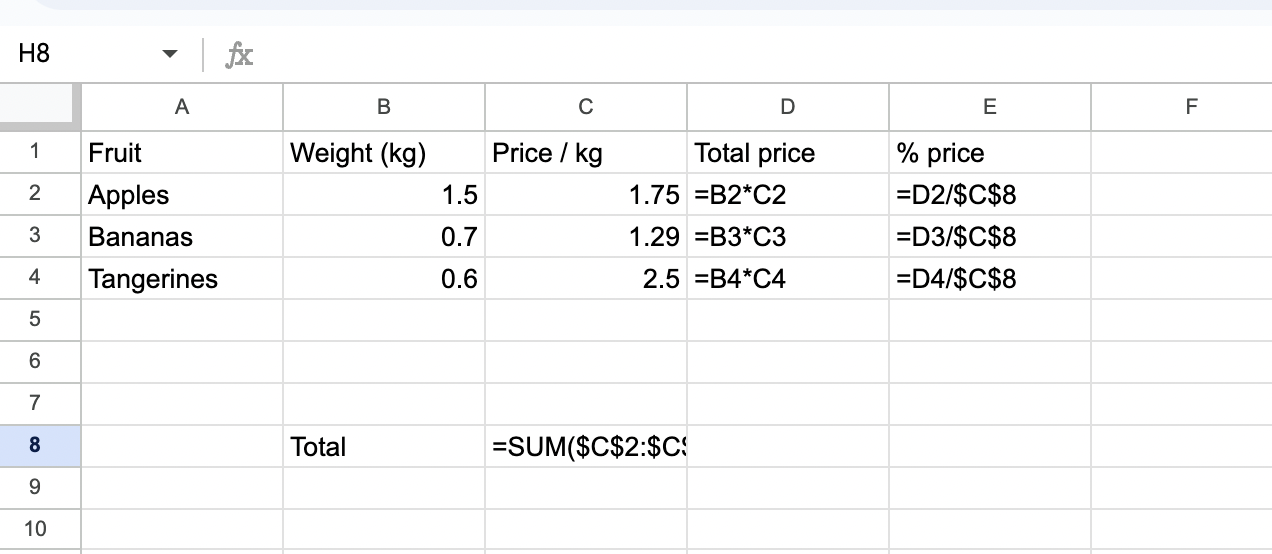
\includegraphics[width=.9\textwidth]{fruit1.5}
    \caption{Formulas}
  \end{figure}
\end{frame}
\begin{frame}[fragile]
  \begin{figure}
    \centering
    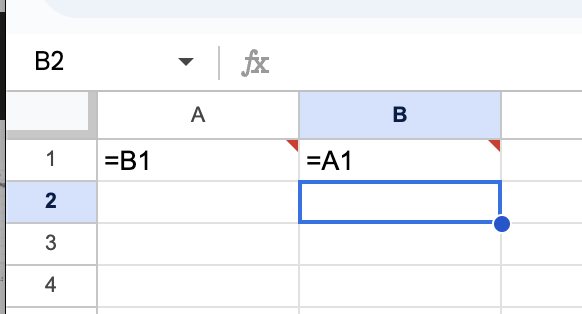
\includegraphics[width=.45\textwidth]{circular_formula}\\
    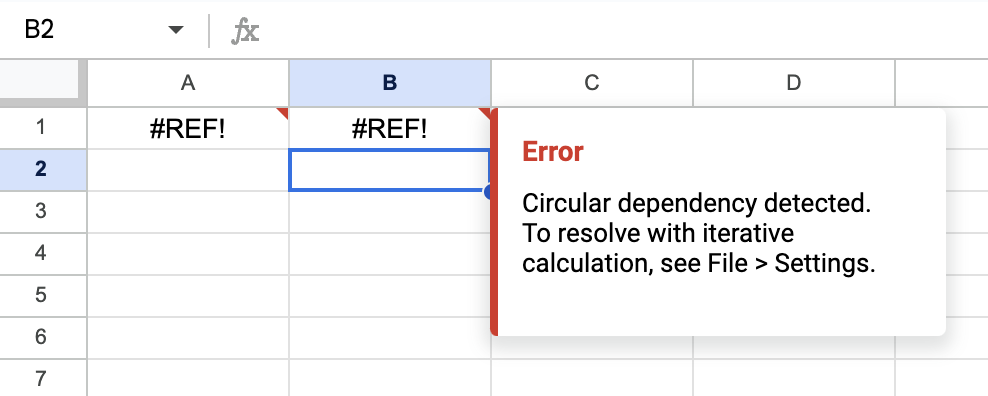
\includegraphics[width=.75\textwidth]{circular}
    \caption{Circular dependencies}
  \end{figure}
\end{frame}

\begin{frame}[fragile]
  \begin{figure}
    \centering
  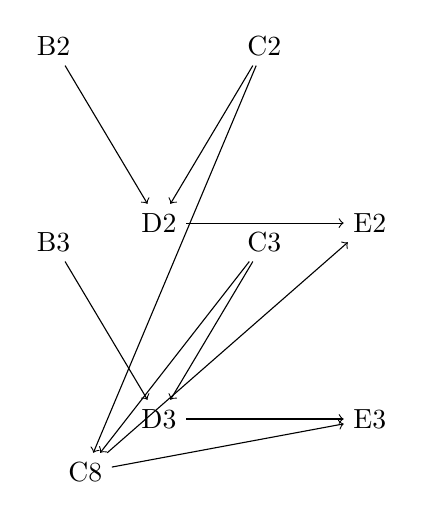
\begin{tikzpicture}[node distance=2cm]
    % Define nodes
    \node (B2) {B2};
    \node (C2) [right=of B2] {C2};
    \node (D2) [below=of $(B2)!0.5!(C2)$] {D2};
    \node (E2) [right=of D2] {E2};

    \node (B3) [below=of B2]{B3};
    \node (C3) [right=of B3] {C3};
    \node (D3) [below=of $(B3)!0.5!(C3)$] {D3};
    \node (E3) [right=of D3] {E3};

    \node (C8) [below=of $(B3)!0.3!(D3)$] {C8};
    % Draw arrows
    \draw[->] (B2) -- (D2);
    \draw[->] (C2) -- (D2);
    \draw[->] (D2) -- (E2);
    
    \draw[->] (B3) -- (D3);
    \draw[->] (C3) -- (D3);
    \draw[->] (D3) -- (E3);
    
    \draw[->] (C8) -- (E2);
    \draw[->] (C8) -- (E3);
    
    \draw[->] (C2) -- (C8);
    \draw[->] (C3) -- (C8);
\end{tikzpicture}
    \caption{DAG}
  \end{figure}
\end{frame}


\begin{frame}[fragile]
 Associated to a spreadsheet is a DAG where
  \begin{itemize}
    \item nodes are cells
    \item there is a directed edge from $a$ to $b$ if and only if $b$ has a formula that depends on $a$ (\ie, $b$ depends on $a$)
  \end{itemize}

\end{frame}

\begin{frame}[fragile]
  Spreadsheet \emph{evaluation} is analogous to \emph{dependency resolution}
 \end{frame}

\begin{frame}[fragile]
  A modern spreadsheet application provides many additional capabilities, not in scope in this talk, such as
  \begin{itemize}
    \item Parsing of cell formulas
    \item Built-in functions
    \item Graphics (\eg, histograms, piecharts, etc) 
    \item Formatting, exporting, drag-and-drop, copy-pasting, etc
    \item Programmable functions (\eg, in VBA) 
    \item Data connectors 
    \item Collaborative online spreadsheets
    \item And many more
  \end{itemize}
\end{frame}


\begin{frame}[fragile]
  \begin{figure}
    \centering
    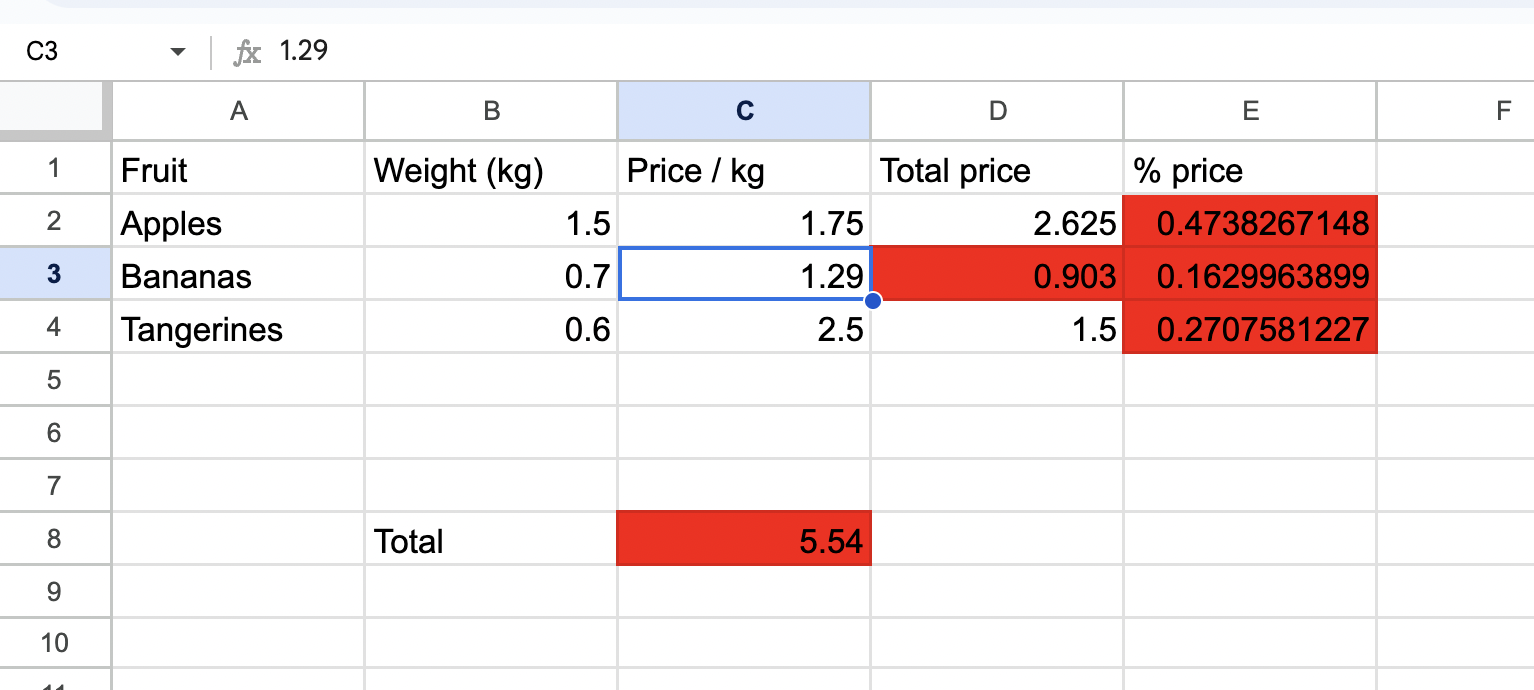
\includegraphics[width=.9\textwidth]{fruit2}
    \caption{Recalculation and support graph}
  \end{figure}
\end{frame}

\begin{frame}[fragile]
  MVP / POC: recalculate the whole spreadsheet every time a cell changes
\end{frame}

\begin{frame}[fragile]
  POST MVP: \emph{incremental recalculation}

  Traditional technique:
  \begin{itemize}
    \item Topological sorting of the support graph%
  \footnote{\url{https://en.wikipedia.org/wiki/Topological_sorting}}
      (\eg, Kahn's algorithm)
  \end{itemize}
\end{frame}

\begin{frame}[fragile]
  Production applications need to take into account more complicated challenges:%
  \footnote{\url{https://learn.microsoft.com/en-us/office/client-developer/excel/excel-recalculation}}
  \begin{itemize}
    \item Performance tradeoffs (\eg, calculating the topological order also has an associated cost) 
    \item Resource utilisation  (\eg, compact representations) 
    \item Volatile functions (\eg, \verb|now()|, \verb|rand()|)
    \item DAG caching 
    \item Parallelisation algorithms, etc
  \end{itemize}
\end{frame}

\begin{frame}[fragile]
  \begin{figure}
    \centering
    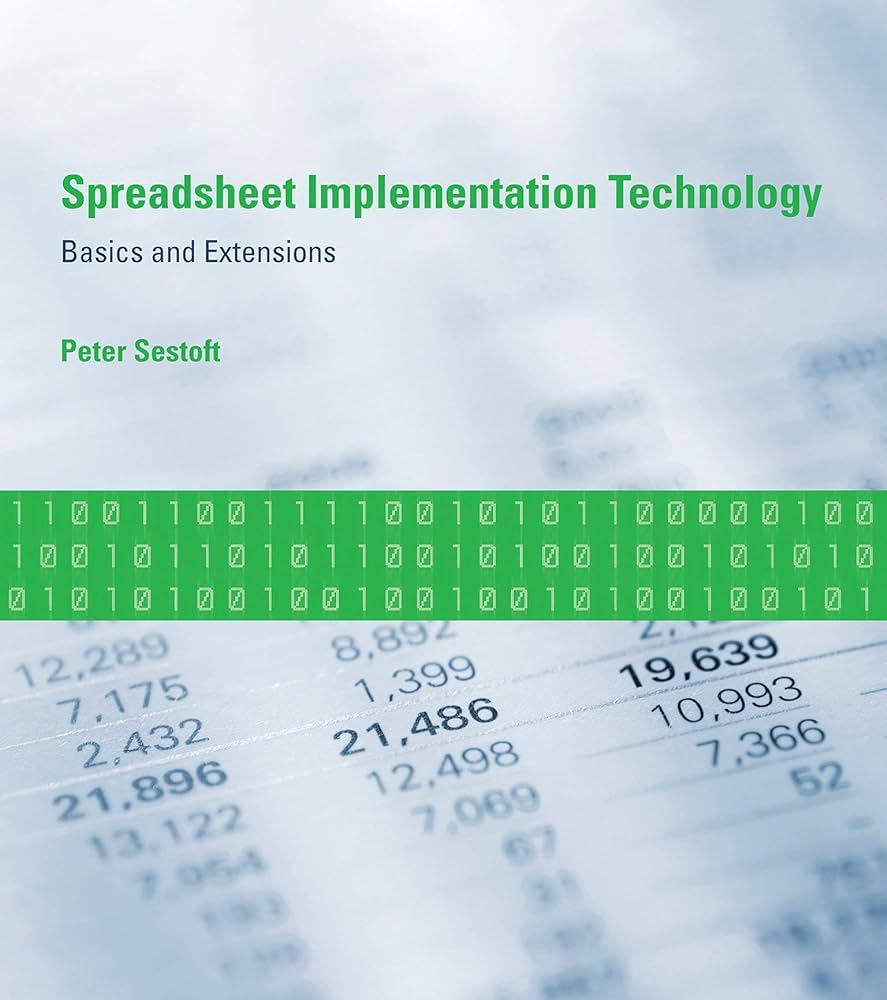
\includegraphics[height=.7\textheight]{cover}
    \caption{P.~Sestoft, \emph{Spreadsheet Implementation Technology}, MIT press (2014).\protect\footnotemark} 
    \footnotetext{\url{https://direct.mit.edu/books/book/3071/Spreadsheet-Implementation-TechnologyBasics-and}}
  \end{figure}
\end{frame}


\begin{frame}[fragile]
  \begin{alertblock}{Observation}
    Spreadsheet-like evaluation can be expressed as a \emph{fixed-point of higher dimensional comonads}
  \end{alertblock}
\end{frame}

\begin{frame}{Agenda}
  \setbeamertemplate{section in toc}[sections numbered]
  \tableofcontents[hideallsubsections]
\end{frame}

\section{A taste of comonads}

\begin{frame}[fragile]
  \begin{figure}
    \centering
    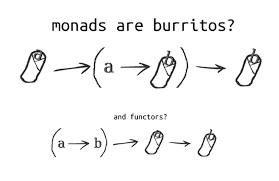
\includegraphics[width=.9\textwidth]{burritos}
    \caption{Monads are burritos}
  \end{figure}
\end{frame}


\begin{frame}[fragile]
  \begin{definition}
    Comonads are co-burritos
  \end{definition}
\end{frame}

\begin{frame}[fragile]
  Functor hierarchy:
  \begin{lstlisting}[language=haskell, basicstyle=\ttfamily]
  class Functor f where 
    fmap :: (a -> b) -> f a -> f b 
  \end{lstlisting}
  %\begin{lstlisting}[language=scala, basicstyle=\ttfamily]
  %trait Functor[F[_]]: 
    %def map[A,B](f : A => B) : F[A] => F[B]
  %\end{lstlisting}

  together with some laws. 
\end{frame}

\begin{frame}[fragile]
  \begin{figure}
    \centering
    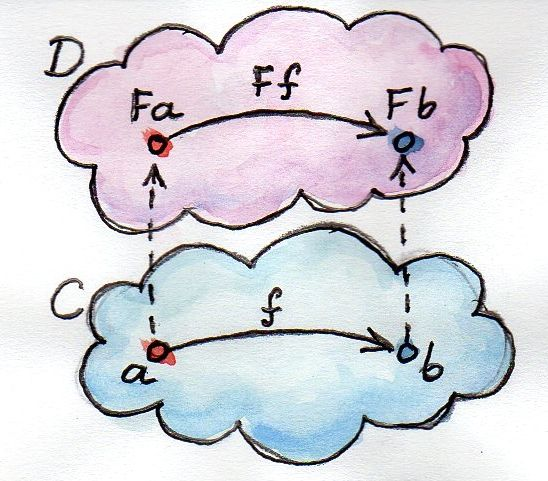
\includegraphics[width=.7\textwidth]{functor}
    \caption{Functors: \emph{Lifting} of 1-ary pure functions to the $f$-world}
  \end{figure}
\end{frame}


\begin{frame}[fragile]
  \begin{lstlisting}[language=haskell, basicstyle=\ttfamily]
  f1 :: [Int] -> [String] 

  -- vs 

  f2 :: Int -> String 

  f3 :: [Int] -> [String]
  f3 = fmap f2
  \end{lstlisting}
\end{frame}


\begin{frame}[fragile]
  \begin{lstlisting}[language=haskell, basicstyle=\ttfamily]
  class (Functor f) => Applicative f where 
    pure :: Applicative f => a -> f a 
    ap :: Applicative f => f (a ->b) -> f a -> f b 
  \end{lstlisting}
  %\begin{lstlisting}[language=scala, basicstyle=\ttfamily]
  %trait Apply[F[_]]: 
    %def ap[A,B](ff : F[A => B]) : F[A] => F[B]
  %trait Applicative[F[_]] extends Apply[F]:// and more 
    %def pure[A](a : A) : F[A]
  %\end{lstlisting}

  together with laws governing properties of \verb|fmap|, \verb|ap|, and \verb|pure|. 

  Applicatives provide lifting of $N$-ary pure functions in the $f$-context

\end{frame}

\begin{frame}[fragile]
  \begin{lstlisting}[language=haskell, basicstyle=\ttfamily]
  class (Applicative f) => Monad f where 
    return :: Monad f => a -> f a 
    join :: Monad f => f (f a) -> f a 
  
  -- flatMap
  bind :: Monad f => m a -> (a -> m b) -> m b 
  \end{lstlisting}
\end{frame}

\begin{frame}[fragile]
  In short:
  \begin{itemize}
    \item Functor $\sim$ \verb|map| 
    \item Applicative $\sim$  \verb|mapN|  (or equivalent) 
    \item Monad $\sim$  \verb|flatMap|  (or equivalent) 
  \end{itemize}

  (and the caveat that the implementation must satisfies certain ``reasonable'' laws that rule out ``unexpected'' behaviours)
\end{frame}

\begin{frame}[fragile]
  This seems very abstract but from a software engineer perspective lifting provides
  \begin{itemize}
    \item Separation of concerns 
    \item Reusability 
    \item Composability 
  \end{itemize}
  
  \verb\flatMap\ ensures no ``callback hell'' of nested effects \verb| f ( f ( f ( ... (f a)  ) )) = f a |
\end{frame}
\begin{frame}[fragile]
  Duality:
  \begin{lstlisting}[language=haskell, basicstyle=\ttfamily]
  class Functor f => Comonad f where 
     coreturn :: f a -> a 
     cojoin :: f a -> f ( f a ) 
  \end{lstlisting}
  (and, as usual, there are important laws) 
\end{frame}

\begin{frame}[fragile]
  \begin{lstlisting}[language=haskell, basicstyle=\ttfamily]
  class Functor w => Comonad w where 
     extract :: f a -> a 
     duplicate :: w a -> w ( w a ) 

  -- coKleisli composition / extract
  coFlatMap :: Comonad w => (w a -> b) -> w a -> w b
  coFlatMap f = fmap f . duplicate
  \end{lstlisting}
  (and, as usual, there are important laws) 
\end{frame}


\begin{frame}[fragile]
  \begin{itemize}
    \item Monadic values are typically \emph{produced} in effectful computations
      \begin{verbatim}
      a -> m b 
      \end{verbatim}
    \item Comonadic values are typically \emph{consumed} in context-sensitive computations (\eg, ``queries'') 
      \begin{verbatim}
      w a -> b
      \end{verbatim}
  \end{itemize}
\end{frame}
\begin{frame}[fragile]
  \verb|Maybe| and \verb|[]| are not comonads (why?)

  \begin{lstlisting}[language=haskell, basicstyle=\ttfamily]
  class Copointed f  where 
     extract :: f a -> a 
  \end{lstlisting}
\end{frame}

\begin{frame}[fragile]
  \begin{lstlisting}[language=haskell, basicstyle=\ttfamily]
  instance Comonad NonEmpty where 
     extract = head 
     duplicate = tails1  
  \end{lstlisting}
\end{frame}


\begin{frame}[fragile]
\begin{lstlisting}[language=haskell, basicstyle=\ttfamily]
{-# LANGUAGE OverloadedLists #-}
-- return all suffices including itself

tails [1,2,3] `shouldBe`
       [[1,2,3], [2, 3], [3]]
  \end{lstlisting}
\end{frame}
    
\begin{frame}[fragile]
\begin{lstlisting}[language=haskell, basicstyle=\ttfamily]
{-# LANGUAGE OverloadedLists #-}
coFlatMap f [1,2,3] `shouldBe`
       [f [1,2,3], f [2, 3], f [3]]

-- in this case
-- coFlatMap f = fmap f . tails 
       
  \end{lstlisting}
\end{frame}

\begin{frame}[fragile]
  Simple moving average of a time series $[\phi_{1}, \ldots, \phi_{N}]$ with window size $k$ at the time $t$ is
  \begin{equation} 
    SMA_{k}(t) = \frac{1}{k} \sum_{j = t - k + 1}^{t} \phi_{j}
  \end{equation}
\end{frame}


\begin{frame}[fragile]
\begin{lstlisting}[language=haskell, basicstyle=\ttfamily]
{-# LANGUAGE OverloadedLists #-}

sma :: Window -> NonEmpty Int -> [Double]

sma 3 [1,2,3,4,5,6,7,8,9,10] `shouldBe`
   [2.0,3.0,4.0,5.0,6.0,7.0,8.0,9.0]
\end{lstlisting}
because 
\begin{itemize}
   \item  
     $(1+2+3) / 3 = 6/3 = 2$
    \item $(2+3+4) / 3 = 9/3 = 3$
    \item $(3+4+5) / 3 = 12/3 = 4$
\end{itemize}
\end{frame}

\begin{frame}[fragile]
\begin{lstlisting}[language=haskell, basicstyle=\ttfamily]
smaLocal :: Window -> NonEmpty Double 
   -> Maybe Double
smaLocal k s = (/ (fromIntegral k)) <$>
        sumK k s

sumFirstK :: Num a => 
   Window -> NonEmpty a -> Maybe a
sumFirstK (Window k) _ | k <= 0 = Nothing
sumFirstK (Window 1) (MyNonEmpty a _) = Just a
sumFirstK k (MyNonEmpty a as) = 
   case nonEmpty as of
     Just as2 -> (+a) <$> sumFirstK (k-1) as
     Nothing -> Nothing
\end{lstlisting}
\end{frame}
\begin{frame}[fragile]
\begin{lstlisting}[language=haskell, basicstyle=\ttfamily]
sma :: Window -> MyNonEmpty Double 
         -> MyNonEmpty (Maybe Double)
sma size = coFlatMap (smaLocal size)
\end{lstlisting}
\end{frame}

\begin{frame}[fragile]
  \begin{alertblock}{Folkloristic understanding of some comonads usages}
    \begin{itemize}
  \item the function passed to \verb|coFlatMap| represents a \emph{local} computation (can explore the ``neighbourhood'' of the focus point, but produces a single value) 
  \item \verb|cojoin| produces a (lazy) view of the structure from all perspectives 
  \item \verb|coFlatMap| applies the local computation to all perspectives 
    \end{itemize}
  \end{alertblock}
\end{frame}
\begin{frame}[fragile]
  Similar examples:
  \begin{itemize}
    \item Numerical derivation
    \item Reconciliation in a list of events
    \item etc
  \end{itemize}
\end{frame}

\begin{frame}[fragile]
  Interesting usages:
  \begin{itemize}
    \item Cellular automaton (\eg, Conway’s game of life)
    \item Store, Moore machine and comonadic UIs
  \end{itemize}
\end{frame}

\section{Comonadic vibes meet spreadsheets}

\begin{frame}[fragile]
\begin{lstlisting}[language=haskell, basicstyle=\ttfamily]
  data Stream a = Stream a (Stream a)
    deriving (Eq, Show,Functor)

  instance Comonad Stream where
     extract (Stream a _) = a
     duplicate s'@(Stream _ as) = 
       Stream s' (duplicate as)
  
\end{lstlisting}
\end{frame}

\begin{frame}[fragile]
\begin{lstlisting}[language=haskell, basicstyle=\ttfamily]
  iterate :: (a -> a) -> a 
    -> Stream a
  iterate f seed = 
    Stream seed (iterate f (f seed))  

  takeN :: Int -> Stream a -> [a] 
  takeN 0 _ = [] 
  takeN n (Stream a as) = a : takeN n as 
\end{lstlisting}
\end{frame}

\begin{frame}[fragile]
\begin{lstlisting}[language=haskell, basicstyle=\ttfamily]
  naturals :: Stream Imt
  naturals = iterate (+1) 0 

  takeN 10 naturals `shouldBe` [0,1,2,3,4,5,6,7,8,9]
\end{lstlisting}
\end{frame}


\begin{frame}[fragile]
  One-dimensional, bidirectional, homogeneous spreadsheet of type $a$
\begin{lstlisting}[language=haskell, basicstyle=\ttfamily]
data Sheet1 = Sheet1 (Stream a) a (Stream a)
   deriving (Eq,Show, Functor)
\end{lstlisting}
\end{frame}

\begin{frame}[fragile]
  \begin{lstlisting}[language=haskell, basicstyle=\ttfamily]
  focus :: Sheet1 a -> a
  focus (Sheet1 _ a _ ) = a

  moveL :: Sheet1 a -> Sheet1 a
  moveL (Sheet1 (Stream a as) focus s) 
     = Sheet1 as a (Stream focus s)
  
  moveR :: Sheet1 a -> Sheet1 a
  moveR (Sheet1 s focus (Stream a as)) 
     = Sheet1 (Stream focus s) a as
  \end{lstlisting}
\end{frame}

\begin{frame}[fragile]
\begin{lstlisting}[language=haskell, basicstyle=\ttfamily]
instance Comonad Sheet1 where
  extract = focus
  duplicate s = 
    Sheet1 (allLeft s) s (allRight s) where 
      allLeft = iterate moveL
      allRight = iterate moveR
\end{lstlisting}
  Duplicate is ``diagonalisation'' (as with other comonads derived from zippers) 
\end{frame}


\begin{frame}[fragile]
  \begin{lstlisting}[language=haskell, basicstyle=\ttfamily]
  naturalsSheet1 :: Sheet1 Int
  naturalsSheet1 = Sheet1 (constS 0) 0 naturals
  \end{lstlisting}
\end{frame}

\begin{frame}[fragile]
  We are looking for sheets of functions:
  \begin{lstlisting}[language=haskell, basicstyle=\ttfamily]
  sheet :: Num a => Sheet1 (Sheet1 a -> a)
  \end{lstlisting}
  and the evaluate function should look like 
  \begin{lstlisting}[language=haskell, basicstyle=\ttfamily]
  evaluate :: Num a => Sheet1 (Sheet1 a -> a) 
    -> Sheet1 a 
  \end{lstlisting}
\end{frame}

\begin{frame}[fragile]
  Comonadic fixed-points at rescue%
  \footnote{Why \texttt{ComonadApply}? We need some ``zippiness'', see references at the end}
  \begin{lstlisting}[language=haskell, basicstyle=\ttfamily]
  kfix :: ComonadApply w => w ( w a -> a ) -> w a 
  \end{lstlisting}
  %where
  %\begin{lstlisting}[language=haskell, basicstyle=\ttfamily]
  %class ComonadApply w where 
    %(<@>) :: w ( a -> b) -> w a -> w b 
  %\end{lstlisting}

\end{frame}
\begin{frame}[fragile]
  \begin{figure}
    \centering
    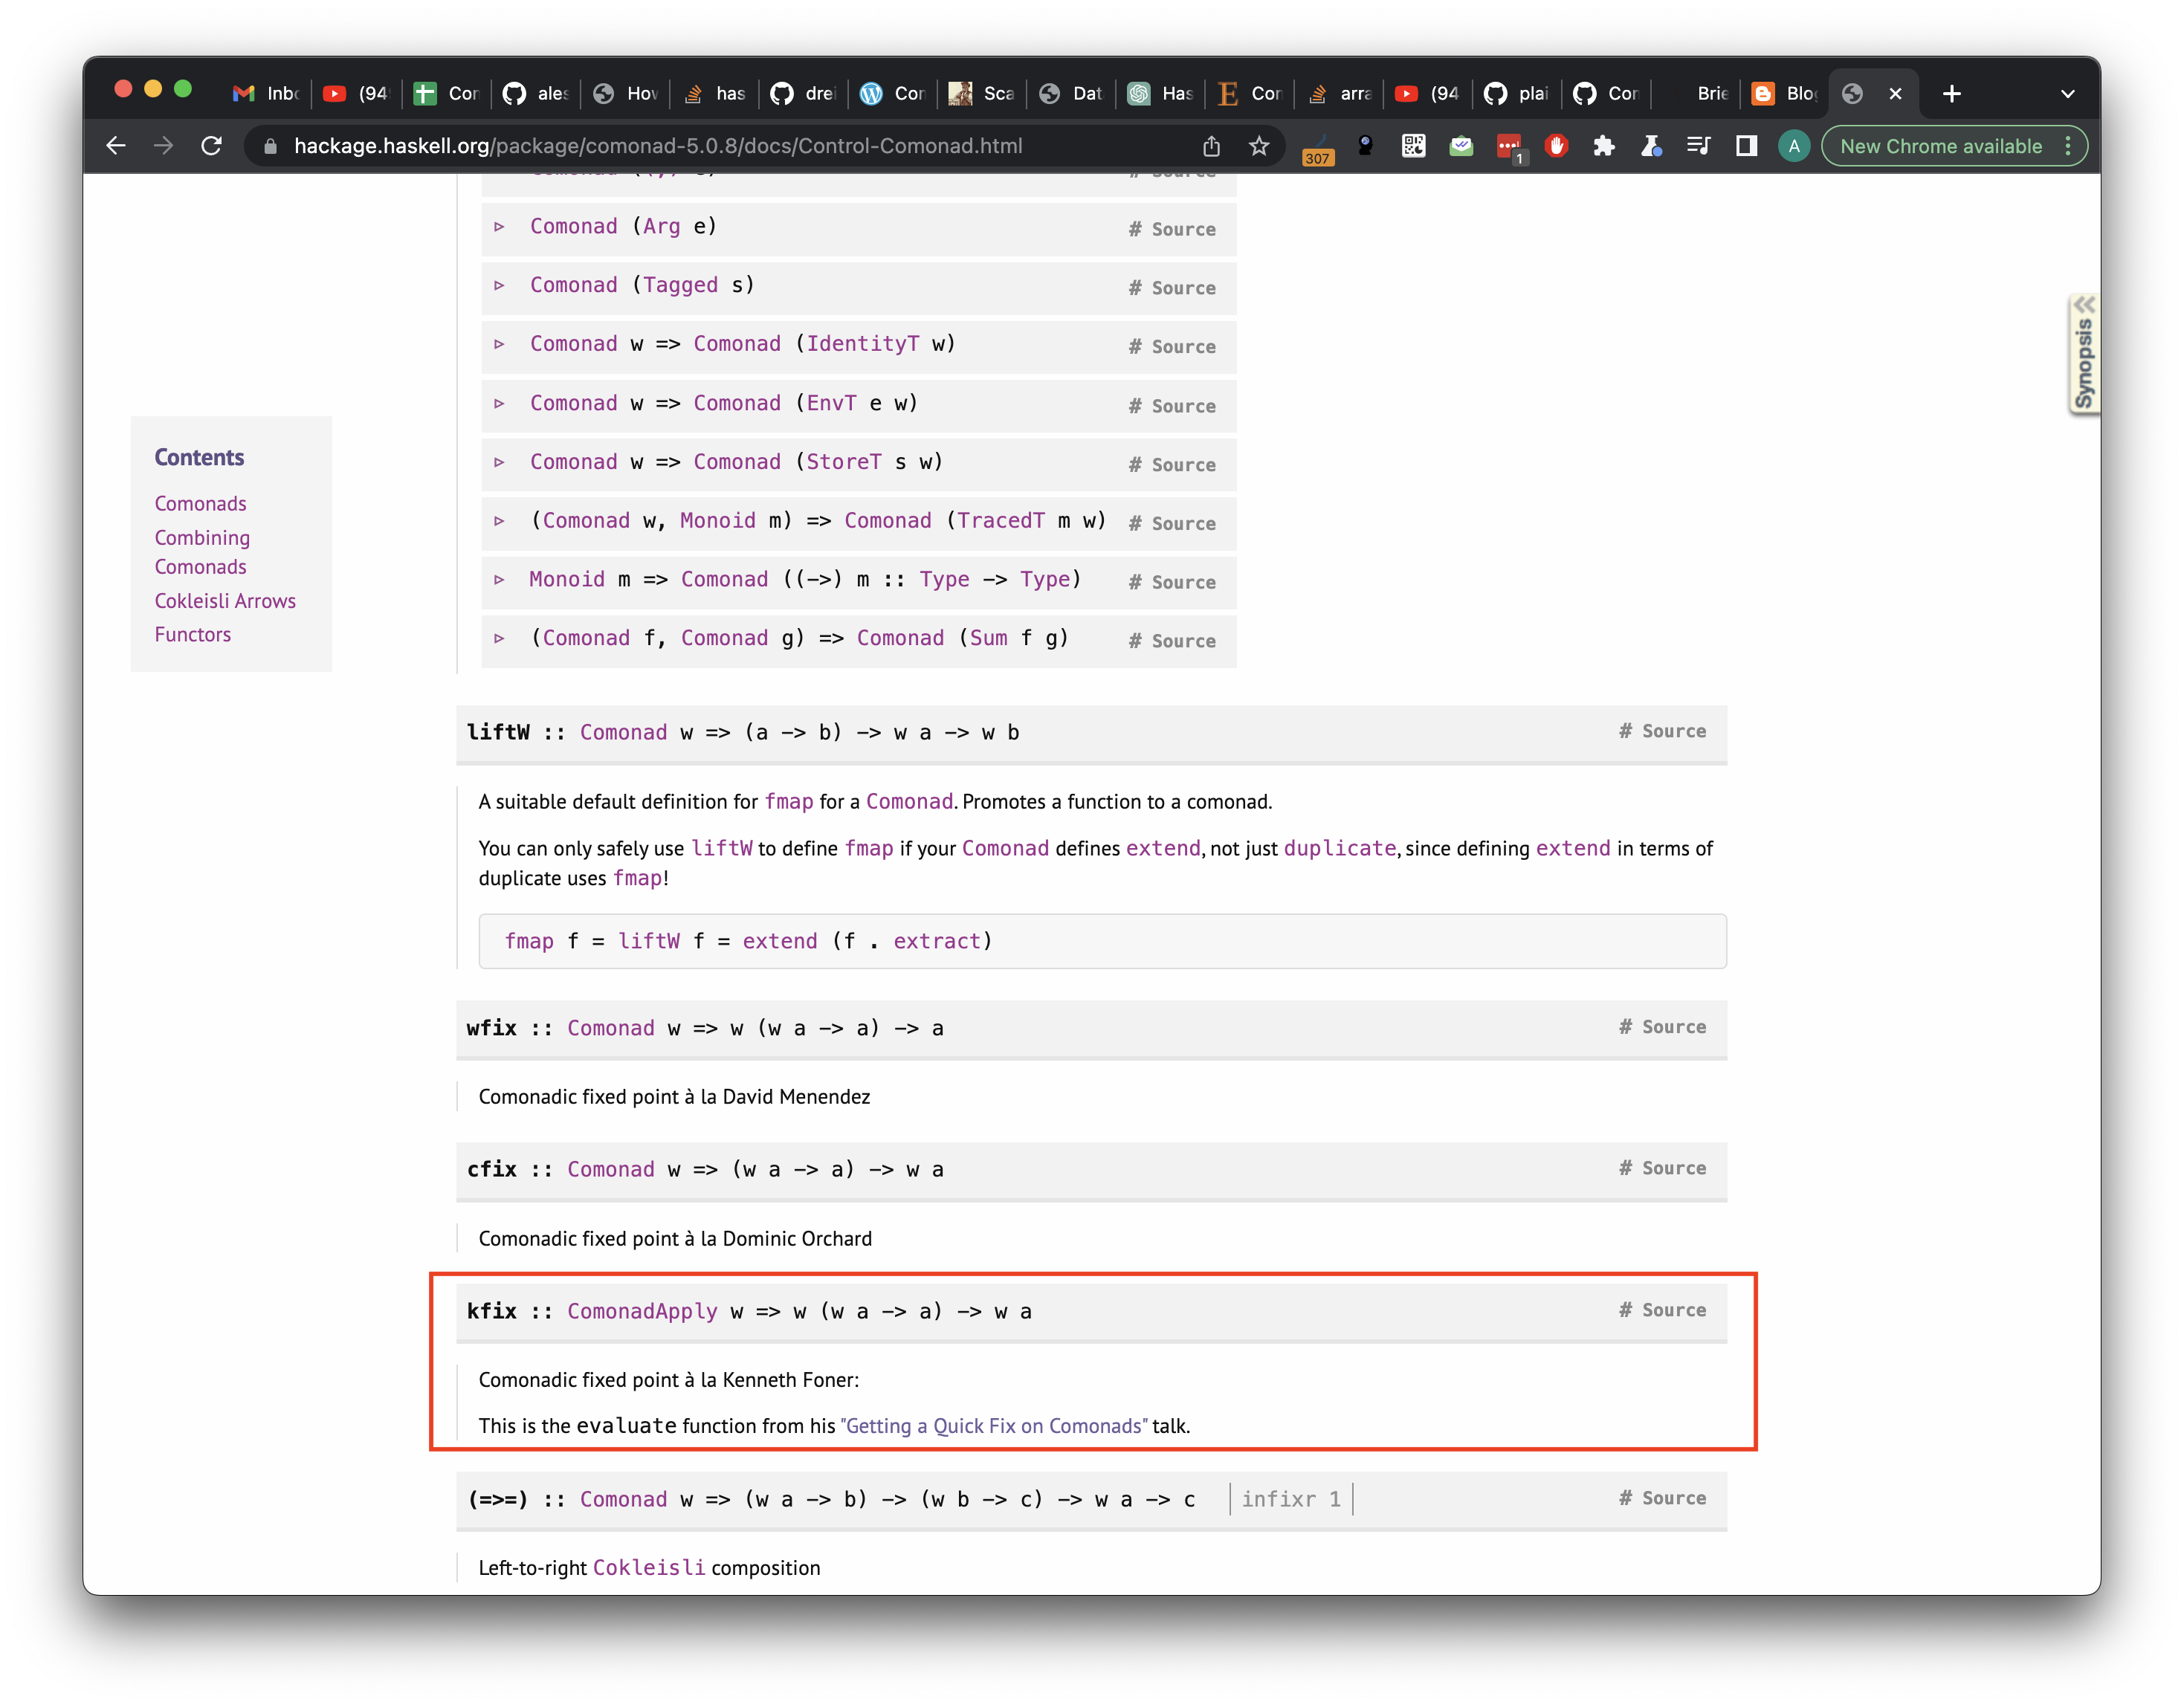
\includegraphics[width=.7\textwidth]{kfix}
    \caption{Kenneth fixed point for \texttt{ComonadApply}}
  \end{figure}
\end{frame}

\begin{frame}[fragile]
  \begin{lstlisting}[language=haskell, basicstyle=\ttfamily]
  \end{lstlisting}
\end{frame}

\begin{frame}[fragile]
  \begin{lstlisting}[language=haskell, basicstyle=\ttfamily]
  \end{lstlisting}
\end{frame}

\begin{frame}[fragile]
\begin{lstlisting}[language=haskell, basicstyle=\ttfamily]
naturals :: Sheet1 Integer
naturals = sheet 0 (repeat (cell left + 1))
\end{lstlisting}
\end{frame}

\section{Down the rabbit hole}

\begin{frame}[fragile]
\begin{figure}
    \centering
    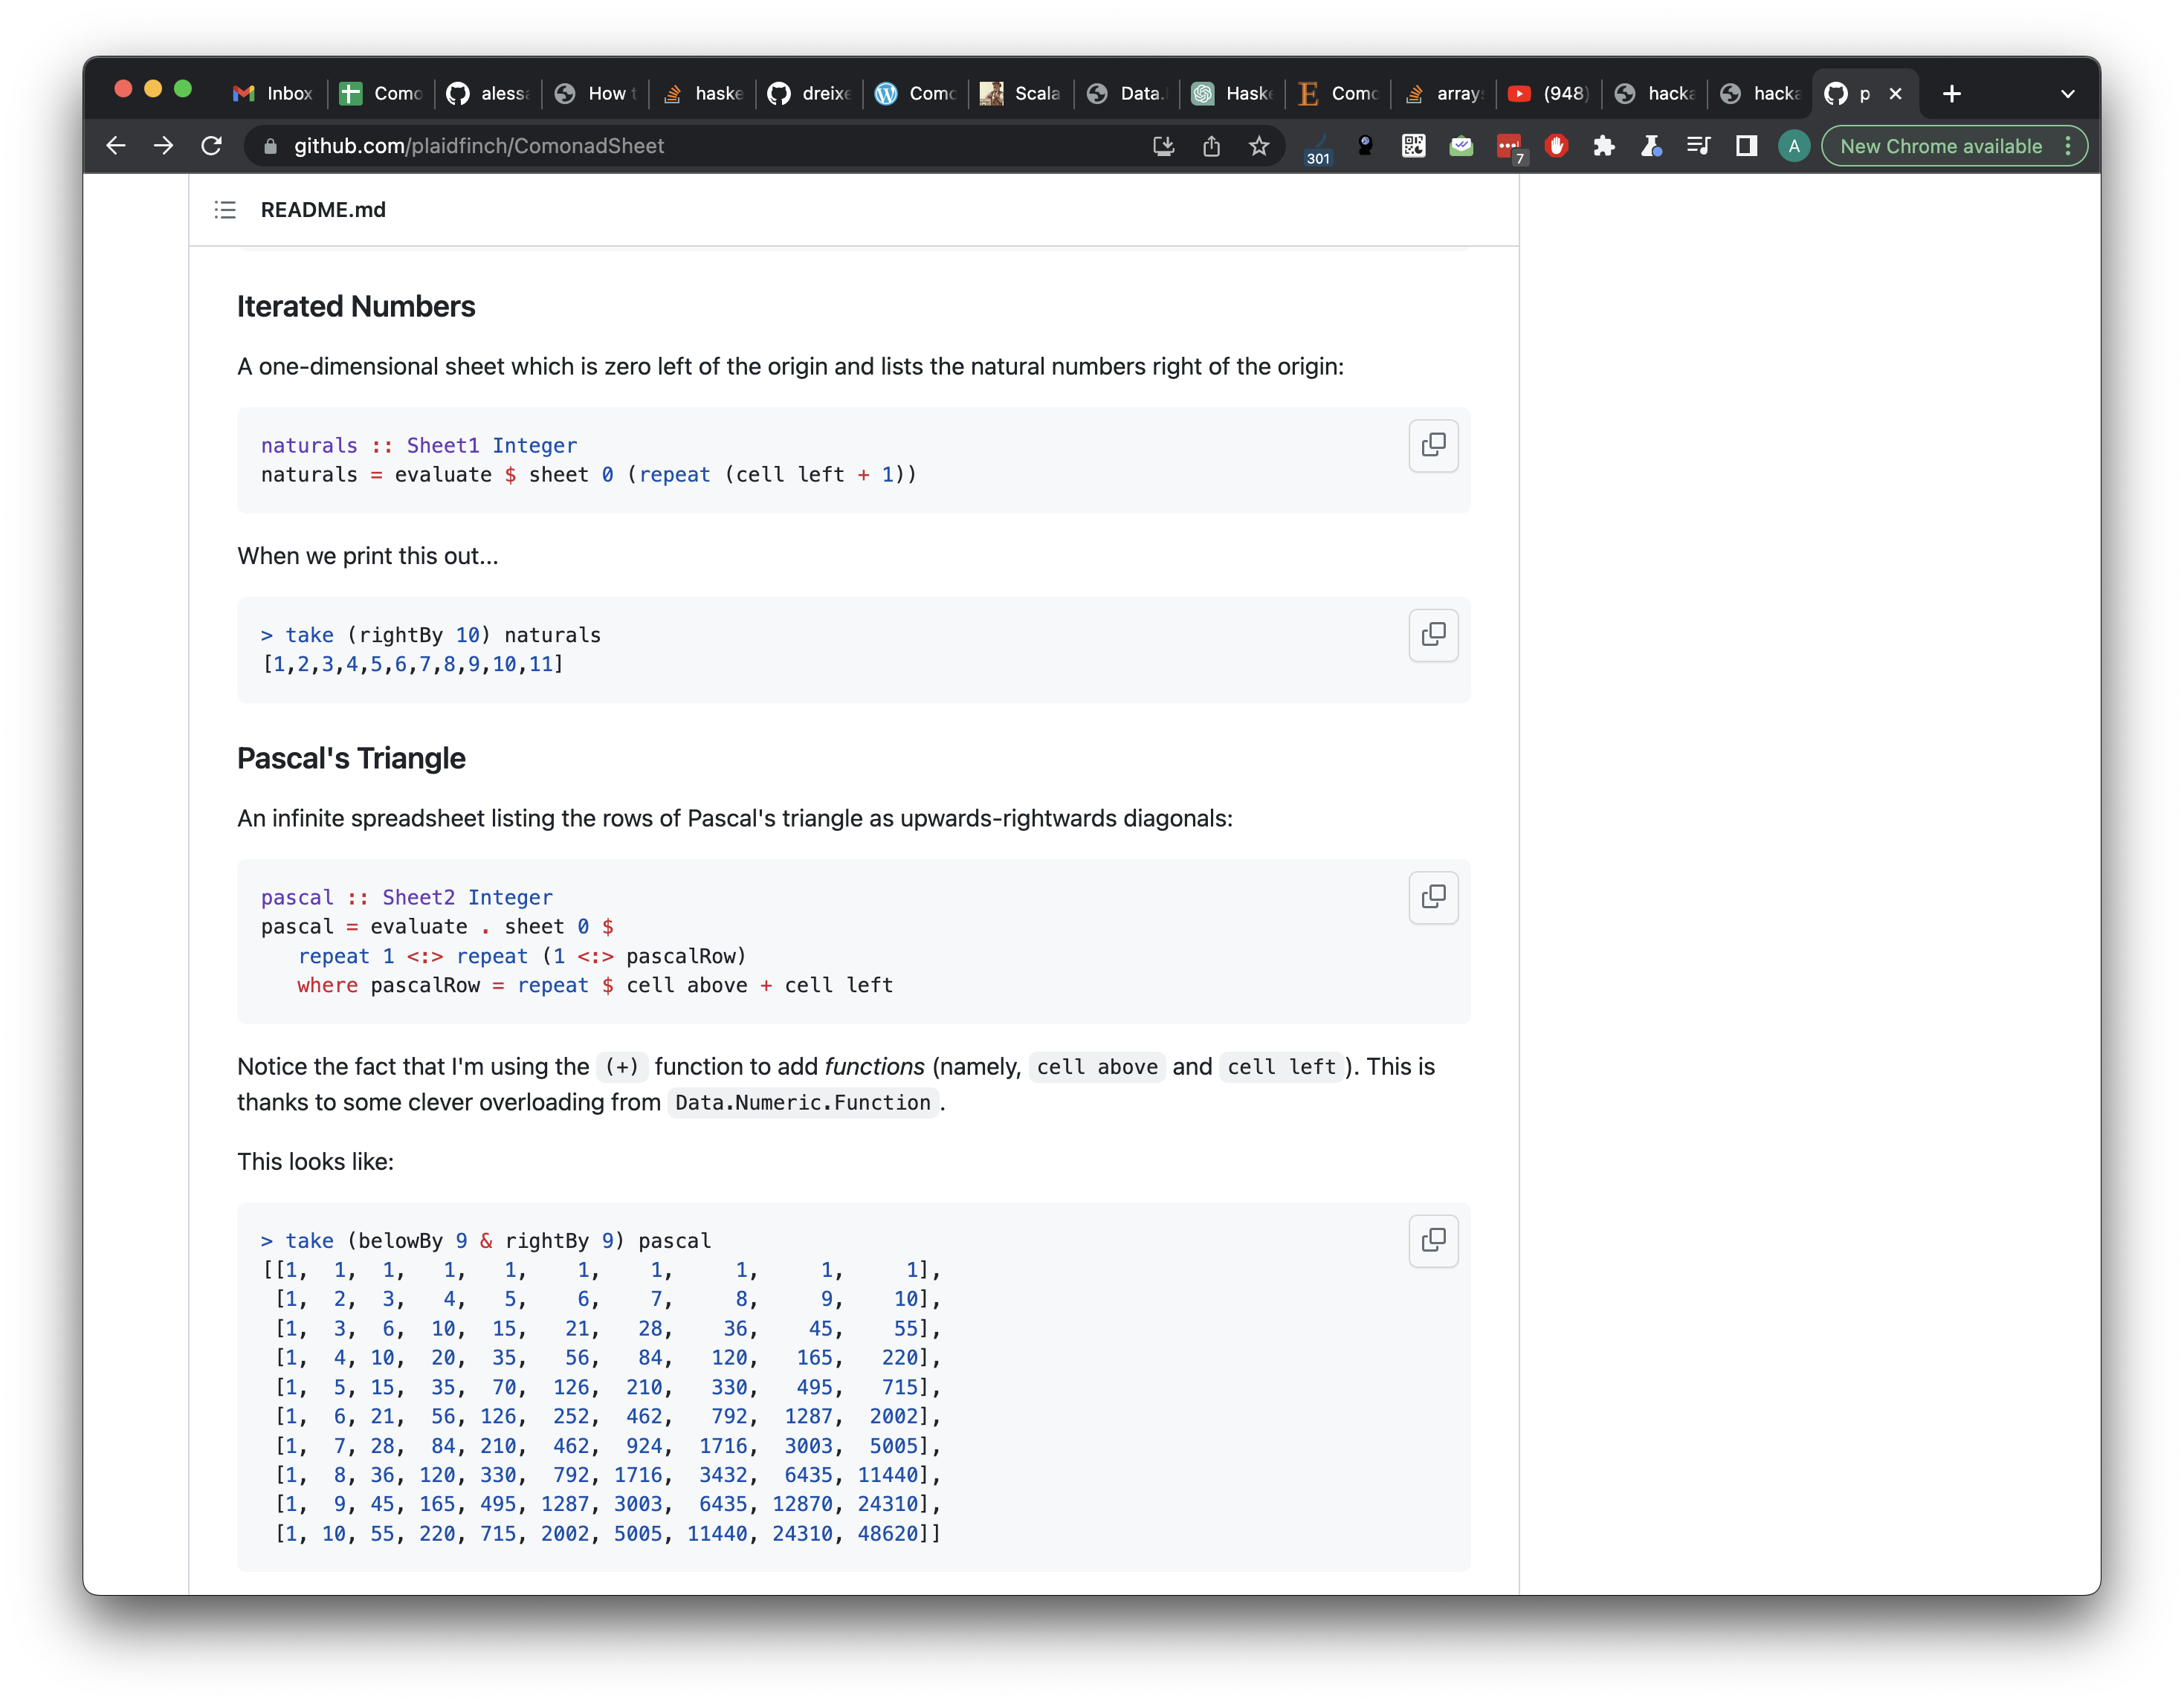
\includegraphics[width=.9\textwidth]{examples}
  \end{figure}
\end{frame}


\begin{frame}[fragile]
  About comonads:
  \begin{itemize}
    \item \url{https://bartoszmilewski.com/2017/01/02/comonads/}
    \item \url{https://blog.higher-order.com/blog/2015/10/04/scala-comonad-tutorial-part-2/}
    \item \url{https://reasonablypolymorphic.com/blog/cofree-comonads/}
    \item \url{https://reasonablypolymorphic.com/blog/comonadic-physics/index.html}
  \end{itemize}
\end{frame}
\begin{frame}[fragile]
  About comonadic UIs:
  \begin{itemize}
    \item \url{https://functorial.com/the-future-is-comonadic/main.pdf}
    \item \url{https://arthurxavierx.github.io/ComonadsForUIs.pdf}
  \end{itemize}
  About cellular automata
  \begin{itemize}
    \item \url{https://www.schoolofhaskell.com/user/edwardk/cellular-automata/part-1} and references therein
  \end{itemize}
\end{frame}


\begin{frame}[fragile]
  From \emph{L\"ob's Theorem} in modal logic%
  \footnote{In this context, $\square \phi$ is a formal provability predicate which reads ``$\phi$ is provable''}
  \begin{equation}
    \square \left( \square \phi \rightarrow \phi \right) \rightarrow \square \phi 
  \end{equation}
  to spreadsheet evaluation:
  \begin{itemize}
    \item Original post from Piponi (2006): \url{http://blog.sigfpe.com/2006/11/from-l-theorem-to-spreadsheet.html}
    \item Functional pearl paper from Kenneth Foner (2015): \url{https://dl.acm.org/doi/10.1145/2887747.2804310}
    \item ComonadSheet hackage package (unmaintained): \url{https://hackage.haskell.org/package/ComonadSheet}
  \end{itemize}
\end{frame}

\plain{Questions?}

%\begin{frame}[allowframebreaks] {References}
% \bibliography{demo}
% \bibliographystyle{abbrv}
%\end{frame}

\end{document}
%% Useful for copy pasting. Would be better to just have snippets
\begin{frame}[fragile]
  \begin{lstlisting}[language=haskell, basicstyle=\ttfamily]
  \end{lstlisting}
\end{frame}
\begin{frame}[fragile]
  \frametitle{}
  \begin{lstlisting}[language=scala, basicstyle=\ttfamily]
  \end{lstlisting}
\end{frame}
